\documentclass{article}

\setlength{\paperwidth}{21cm}   % A4
\setlength{\paperheight}{29.7cm}% A4
\setlength\topmargin{-0.5cm}    
\setlength\oddsidemargin{0cm}   
\setlength\textheight{24.7cm} 
\setlength\textwidth{16.0cm}
\setlength\columnsep{0.6cm}  
\newlength\titlebox 
\setlength\titlebox{5cm}
\setlength\headheight{5pt}   
\setlength\headsep{0pt}
\pagestyle{plain}
\usepackage[dvipsnames]{xcolor}
\usepackage[english]{babel}
\usepackage[nottoc]{tocbibind}
\usepackage{xurl}
\usepackage[colorlinks,citecolor=blue,urlcolor=blue, linkcolor=black, bookmarks=false,hypertexnames=true]{hyperref}
\usepackage{url}
%\usepackage{libertine}
\usepackage{float,multicol}
\usepackage[toc,page]{appendix}
\usepackage{graphicx, subcaption, caption}
\usepackage{doi} % hyperlink URLs
\renewcommand{\doi}{DOI:~}

\newcommand\outauthor{
	\begin{tabular}[t]{c}
		\bf\@author
	\end{tabular}
}

%Add keyword command
\providecommand{\keywords}[1]
{\small\textbf{Keywords:} #1 }

\providecommand{\authorroles}[1]
{\small\textbf{Author roles:} #1 }


\usepackage[english]{babel}
\usepackage[nottoc]{tocbibind}
\usepackage[utf8]{inputenc}
\usepackage{amsmath,amsthm,amsfonts,amssymb,amscd, mathtools, bbm}
\usepackage{lastpage}
\usepackage{enumerate}
\usepackage{fancyhdr}
\usepackage{mathrsfs}
\usepackage{graphicx, wrapfig, lipsum}
\usepackage{listings}
\usepackage{hyperref}
\usepackage{centernot}

\newtheorem{theorem}{Theorem}
\newtheorem{fact}{Fact}
\newcommand{\ra}{\rightarrow}
\newcommand{\sse}{\subseteq}
\let\Pr\relax
\DeclareMathOperator{\Pr}{\mathbb{P}}

\title{\vspace{-50pt} Estimating the Volatility of Returns}

\author{Aditya Raut}

\date{November 5th, 2023}  

\begin{document}
	
\maketitle
\tableofcontents

\section{Task description}
The provided data set contains prices of $6$ stocks named $a$ through $f$, sampled over the course of one year at 1 minute intervals. Our goal in this exercise is to estimate the volatility of these stocks over the month following given data, in the metric of ``annualized percent returns". There are a multitude of choices to be made on how the data is processed, the metrics chosen for returns calculation, sub-sampling or aggregating with a different frequency for training, addition of statistical or time series features, choice of model and validation to name a few. We will make use of highly cited papers on the subject and incorporate the observations and conclusions they have derived about datasets depicting stock prices. We make certain assumptions along the way, which will be highlighted in this report.

\section{Preliminaries}

\begin{itemize}
	\item For an investment of value $V_i$ which grows to a value $V_f$ over a time period, the \textit{return} or \textit{holding period return} can be calculated as $R = \frac{V_f-V_i}{V_i} = \frac{V_f}{V_i}-1$. A popular alternative is \textit{logarithmic return}, calculated by $R_\text{log} = \log\left(\frac{V_f}{V_i}\right)$.\cite{enwiki:1178339248}
	\item Volatility is the degree of variation of trading price over time, usually measured by the standard deviation of logarithmic returns. Annualization of volatility over a period of length $T$, is multiplication by $\sqrt{N}$, if one year consists of $N$ periods of length $T$. \cite{enwiki:1182638071}
\end{itemize}

\section{Data cleaning and exploration}

Over the course of 1 year, there are 252 trading days and the trading time horizon is from 9:30 am to 4:00 pm, which are 391 different minute instances. The data set has $98352$ rows. Plotting the prices for all 6 stocks brings a problem to attention, that some values for stocks $a$ and $d$ are inconsistent and cause huge fluctuations as seen in figure \ref{fig1}. Upon further inspection, they are rogue observations with values $0$ and $1$ for the two stocks respectively, and occur with very small frequency. We remove them and fill any missing values for all stocks with \textbf{the previous timestamp's value} in the data set. This is our \underline{first assumption}, that filling data with 1 minute prior data (or last available timestamp) is reasonable.

\begin{figure}[htb]
	\begin{minipage}{0.5\textwidth}
		\centering
		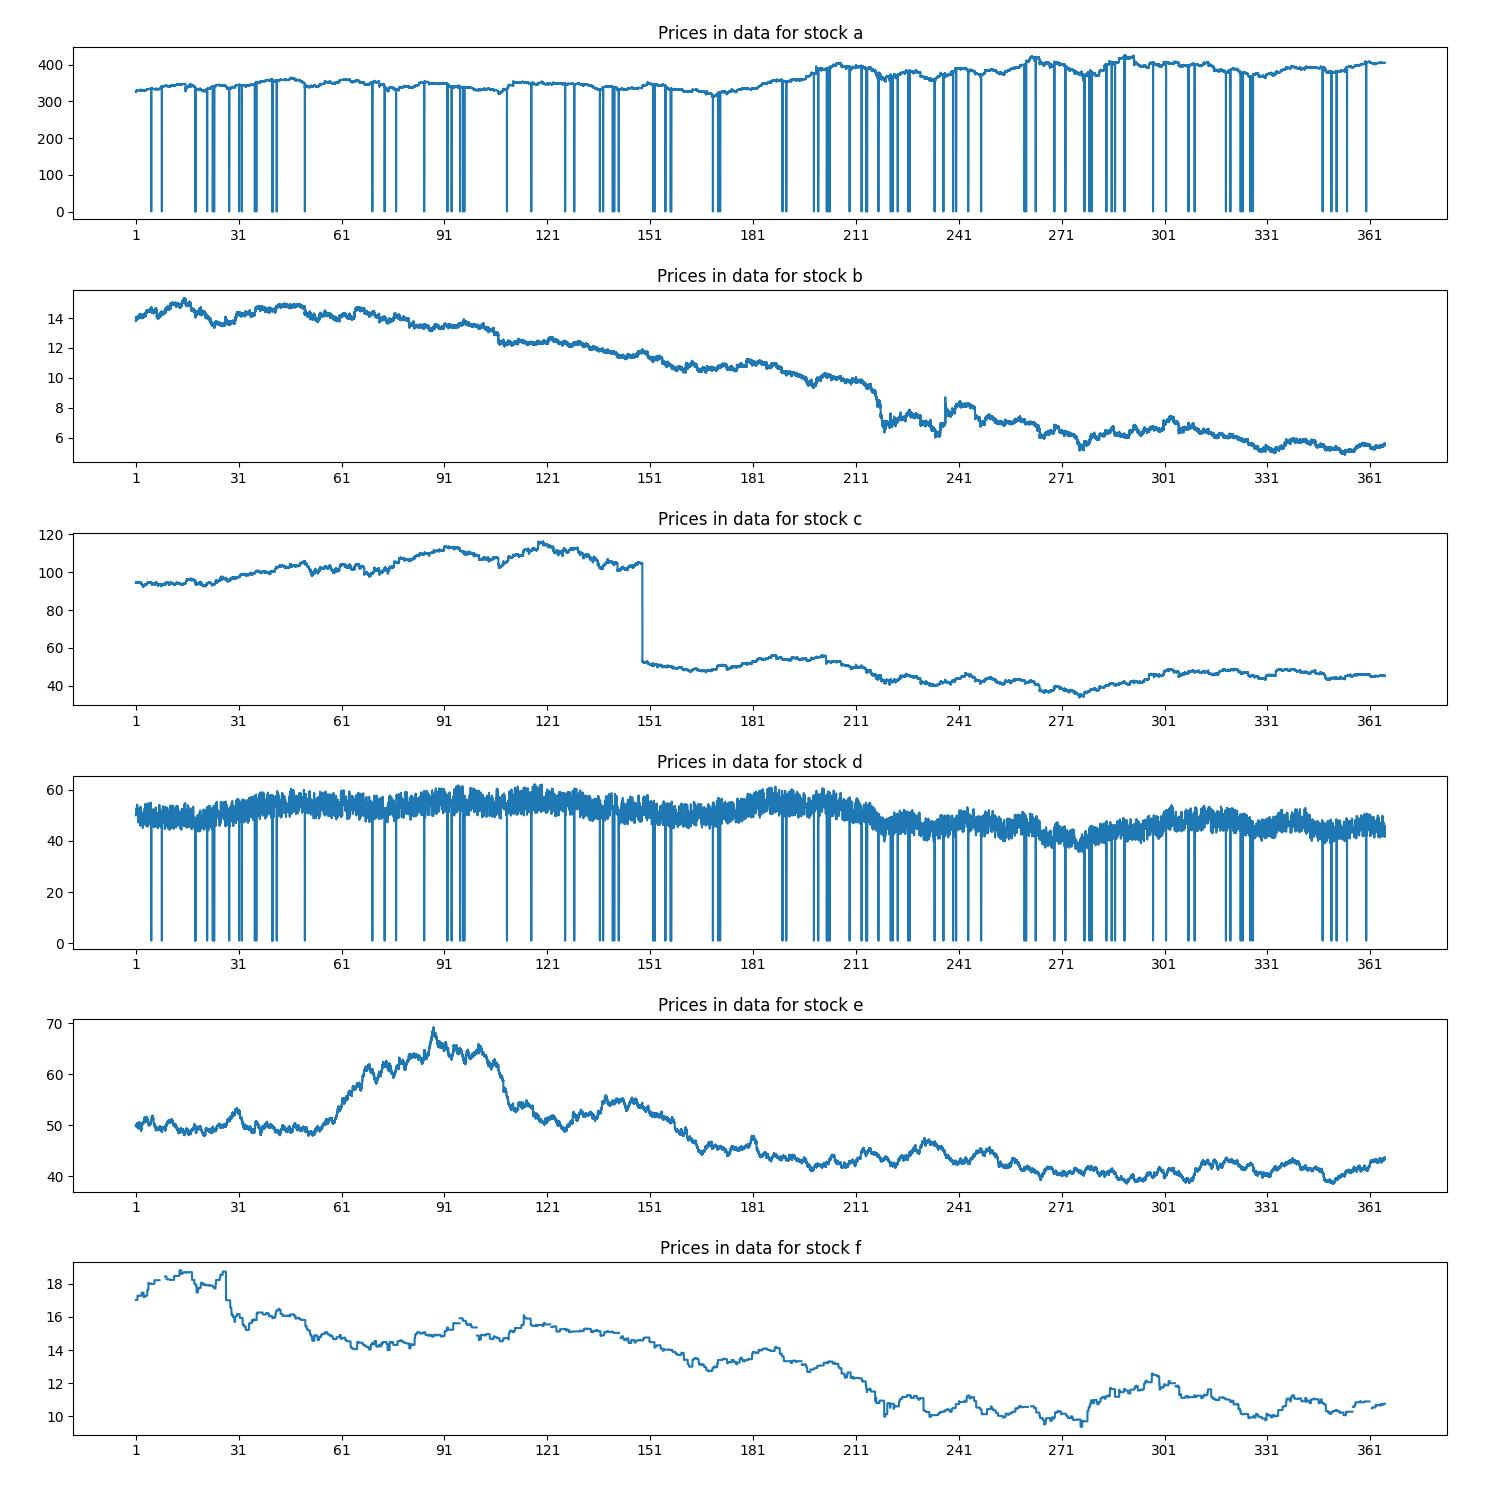
\includegraphics[width=0.8\textwidth, height=0.8\textwidth]{raw_data.jpg}
		\caption{Raw data before any imputation}
		\label{fig1}
	\end{minipage}
	\begin{minipage}{0.5\textwidth}
		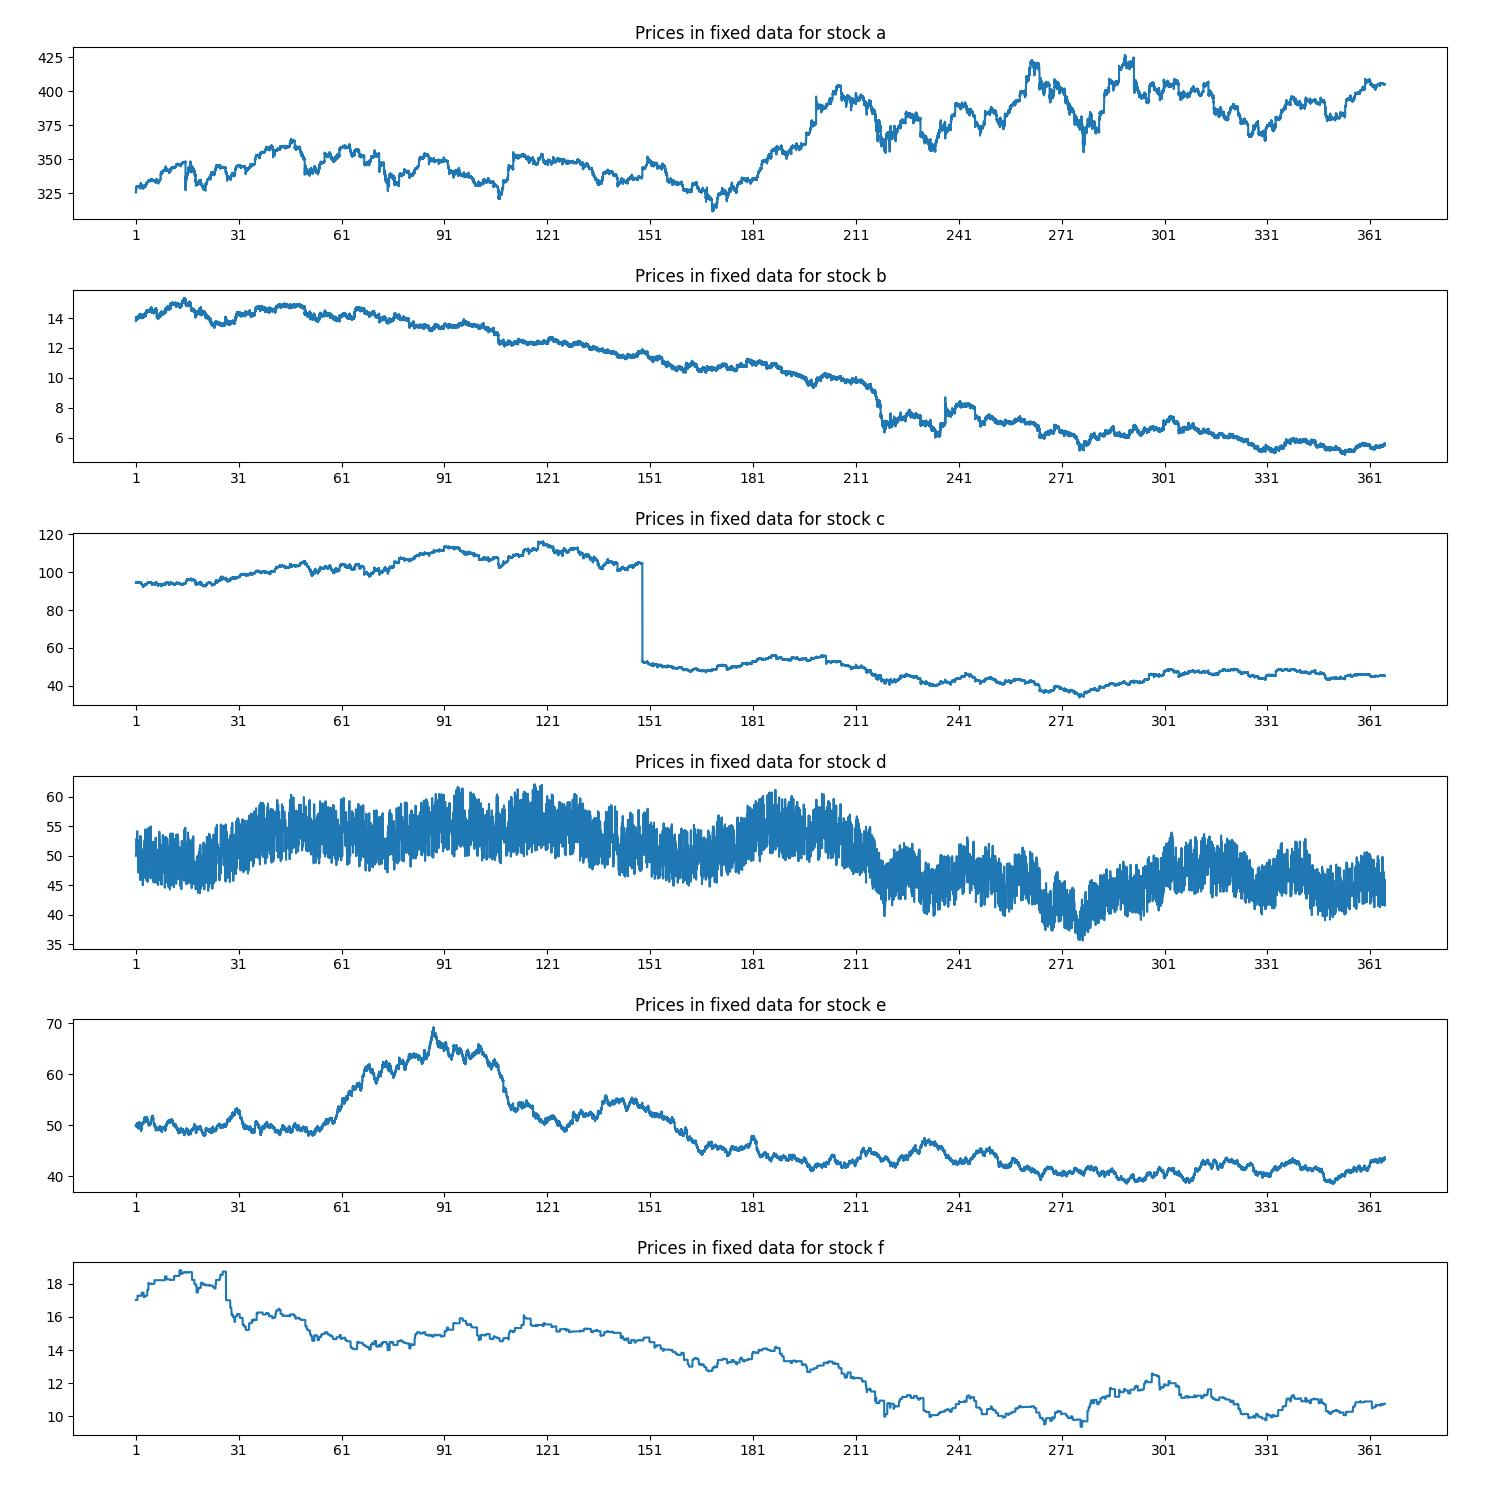
\includegraphics[width=0.8\textwidth, height=0.8\textwidth]{fixed_data.jpg}
		\caption{Fixed data after forward filling}
		\label{fig2}
	\end{minipage}
\end{figure}

The cleaned data more closely resembles usual stock price graphs. We observe that $d$ stock has high daily fluctuations, making it appear much denser than the rest.  

\subsection{Moving average and scatter plots}
We then proceed to plot some moving averages over periods of 1 week to detect time-dependent trends for all the stocks. There are no obvious linear or polynomial trends, with the exception of stock $b$ which follows a linear trend in some part. This is shown in figure \ref{fig3}. We also make scatter plots of pairwise stock prices to find potentially correlated stocks. These initial explorations help us navigate through many options of potential features to be added for predicting this time series, such as time dummies or lag variables. Some scatter plots in figure \ref{fig4} propose some clustered values, implying some dependence. 

\begin{figure}[htb]
	\begin{minipage}{0.5\textwidth}
		\centering
		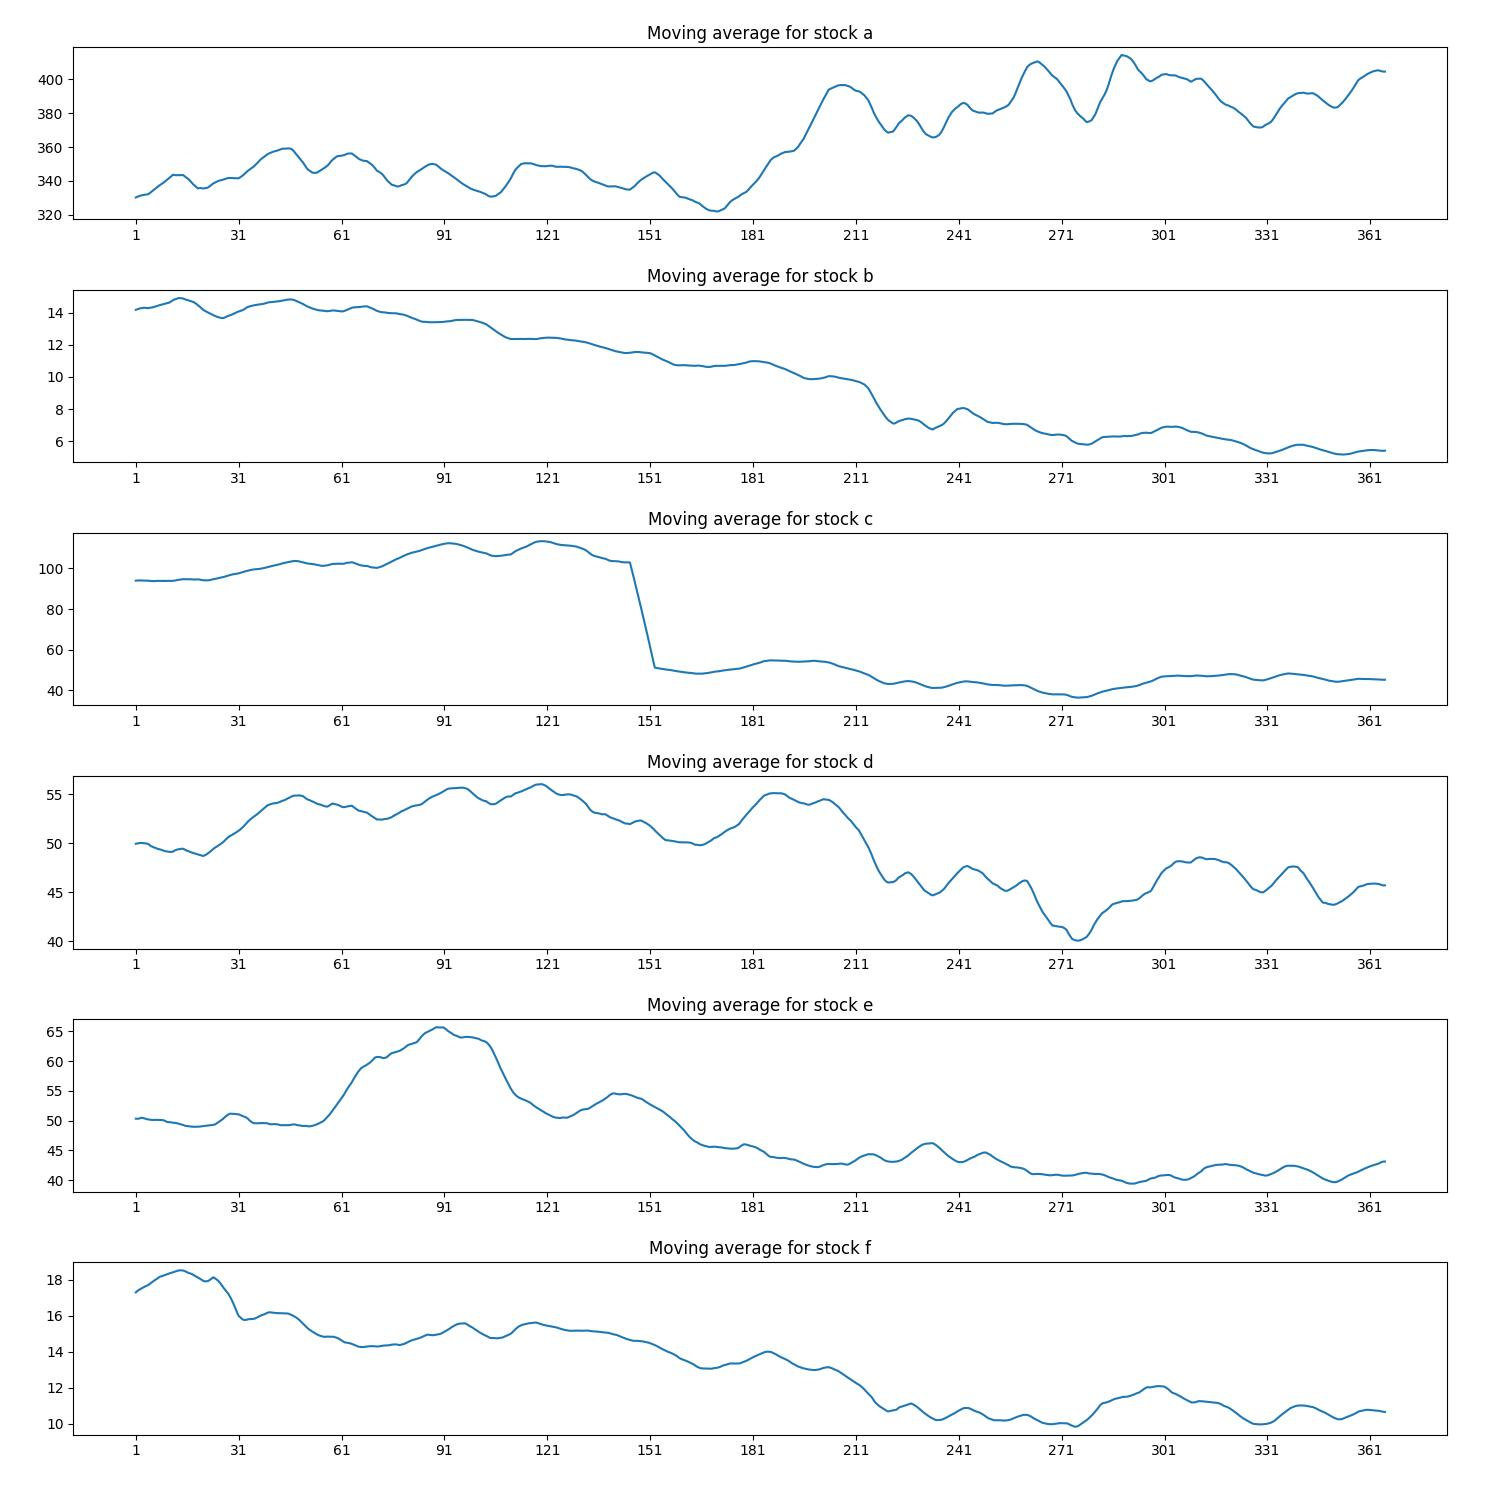
\includegraphics[width=0.8\textwidth, height=0.8\textwidth]{moving_average.jpg}
		\caption{Moving average plot to detect trends}
		\label{fig3}
	\end{minipage}
	\begin{minipage}{0.5\textwidth}
		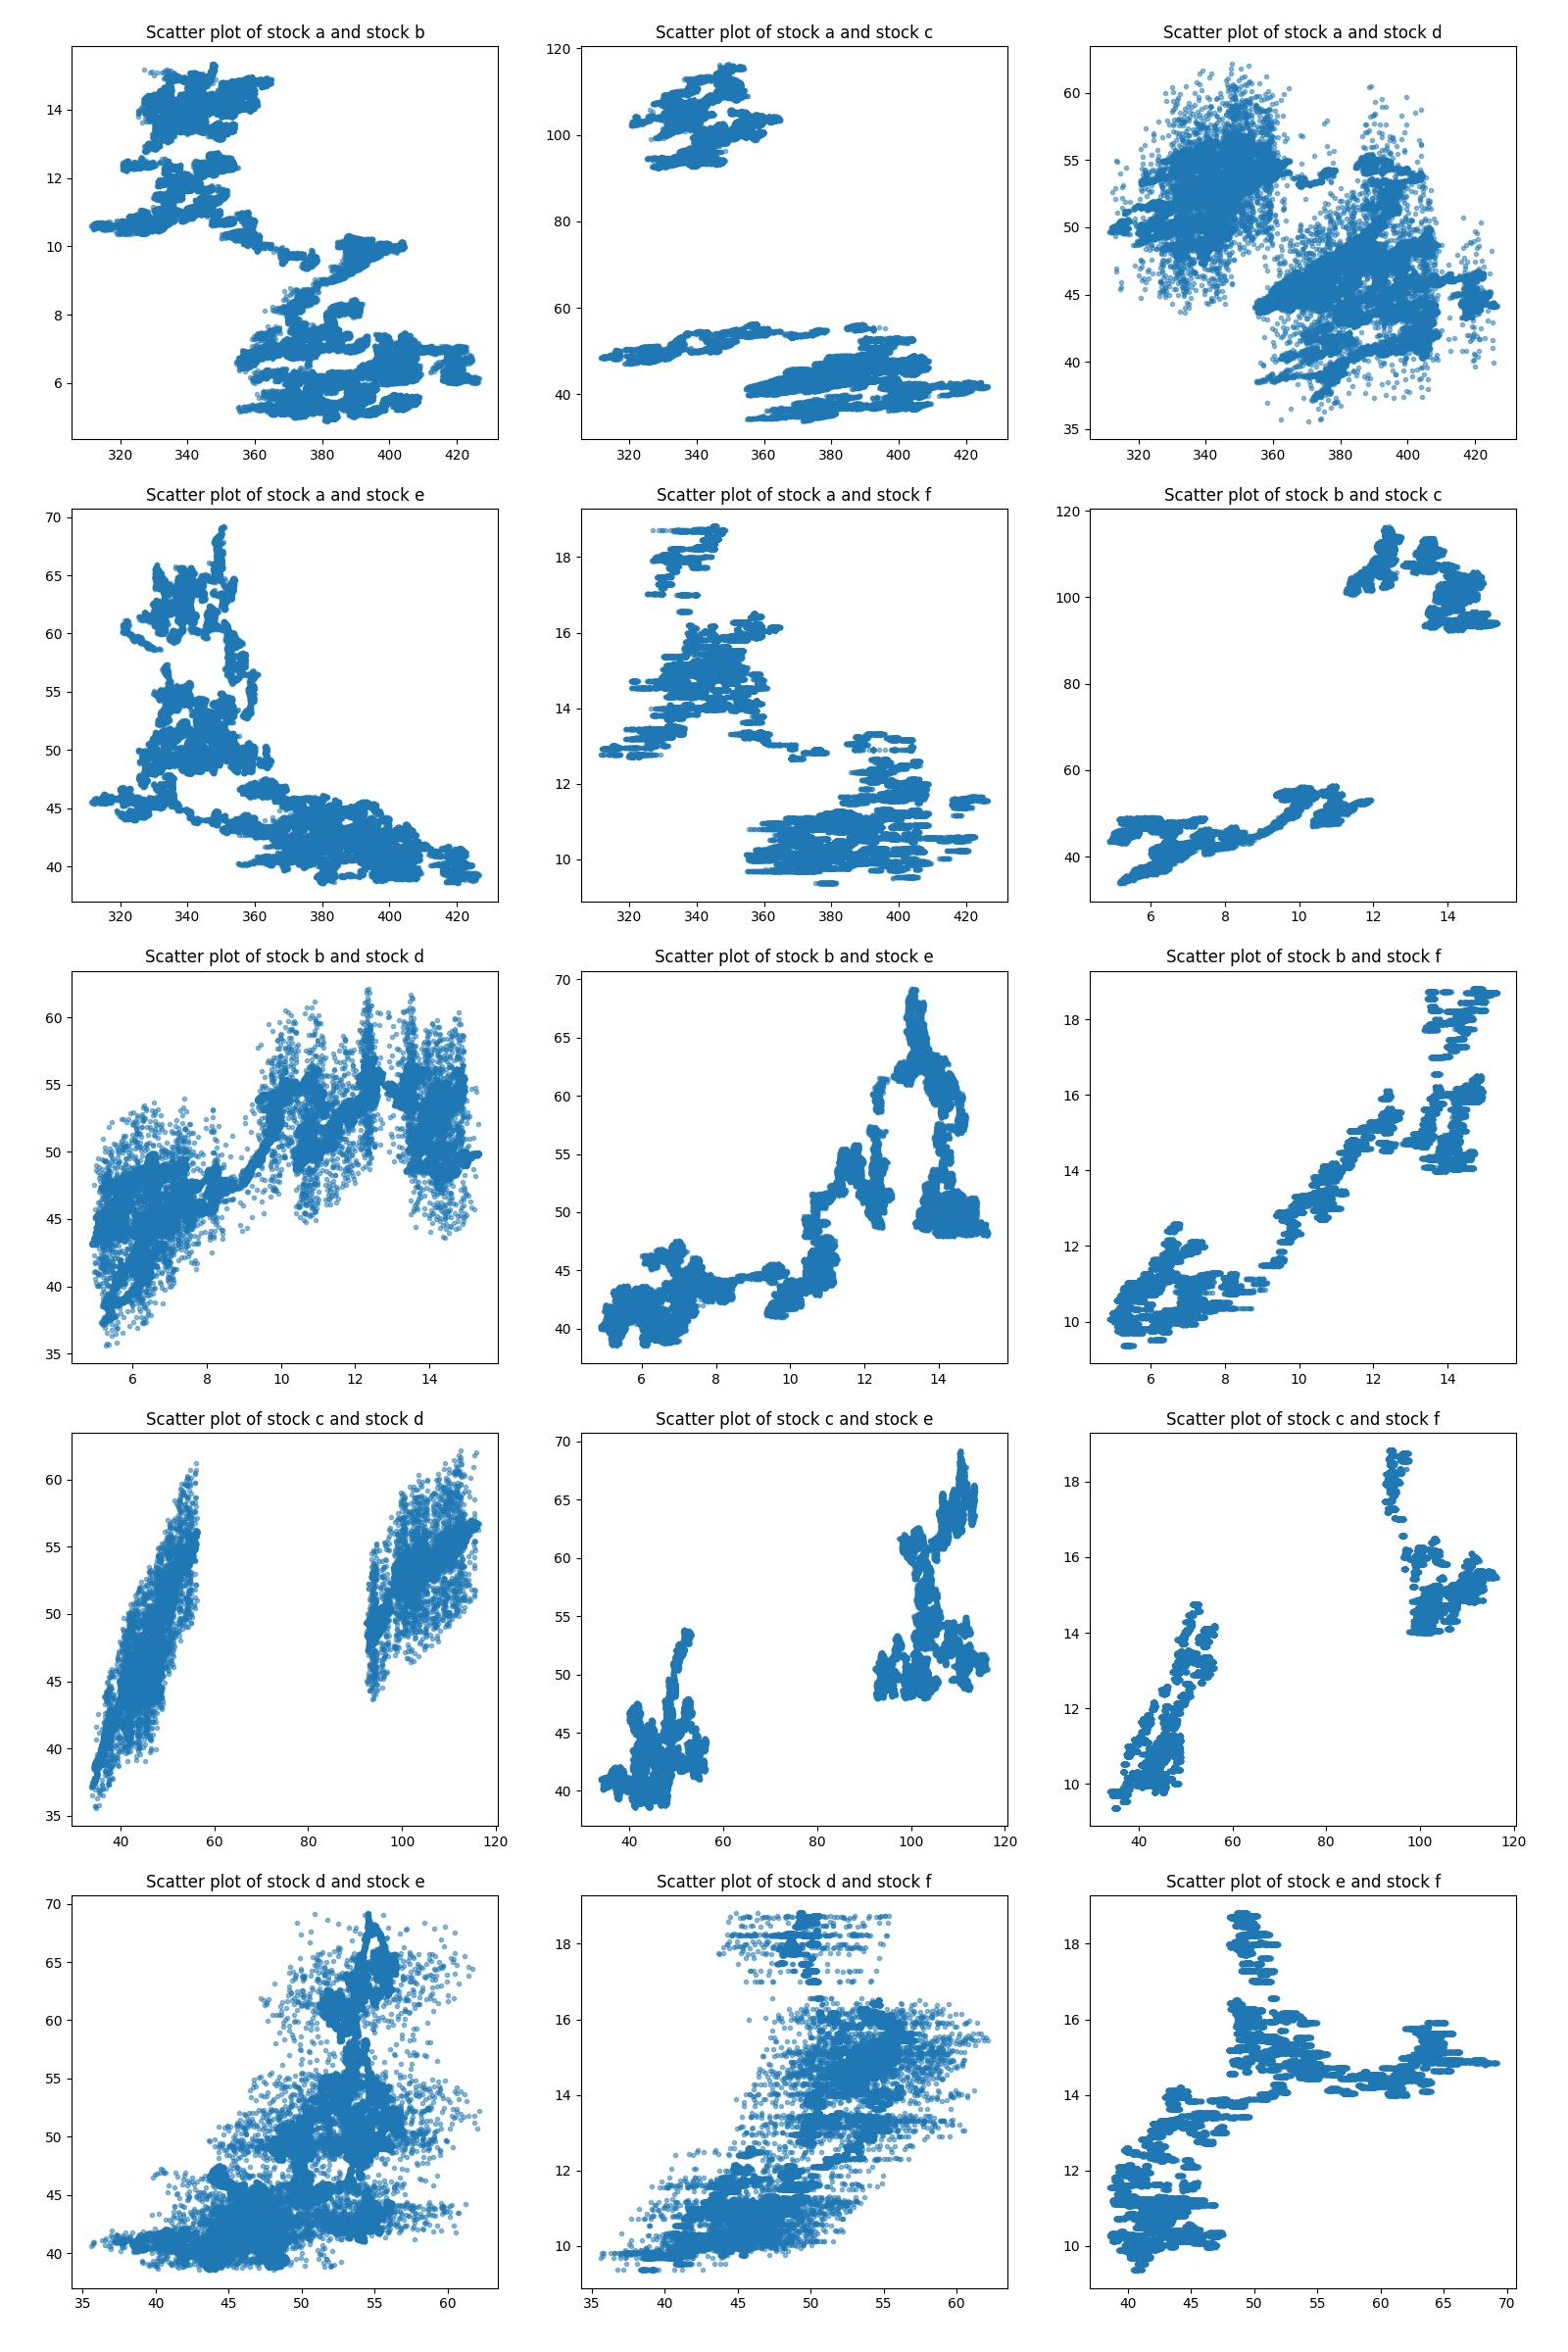
\includegraphics[width=0.8\textwidth, height=0.8\textwidth]{pairwise_scatter.jpg}
		\caption{Pairwise scatter plots of all stocks}
		\label{fig4}
	\end{minipage}
\end{figure}

\section{Data modification}
\subsection{Aggregation to reduce frequency}
While surveying related highly cited literature, we came across the results in \cite{ghysels2006predicting} which state that the direct use of high-frequency data does not improve volatility predictions. This forms the \underline{third assumption} of our approach, motivating aggregation of data at a day level frequency, significantly reducing the number of rows and hence training time and complexity. We use `pandas groupby' method for this. Seeing the distribution of daily price ranges, we observe that its variation is very low on most stocks.

\subsection{Choice of price to consider}
Above aggregation motivates 3 obvious choices for day level aggregation of stock prices, namely the opening, closing and average price. These are defined as the price at 9:30 am, at 4:00 pm and the mean price in that day, respectively. We plot pairwise scatter plots of these 3 prices for all 6 stocks, to observe that they are highly correlated as seen in \ref{fig5}. This leads to our \underline{fourth assumption}, that we can simply consider one of the three prices moving forward. In our analysis, we stick to using \textbf{average daily price}. 

\begin{figure}[htb]
	\centering
	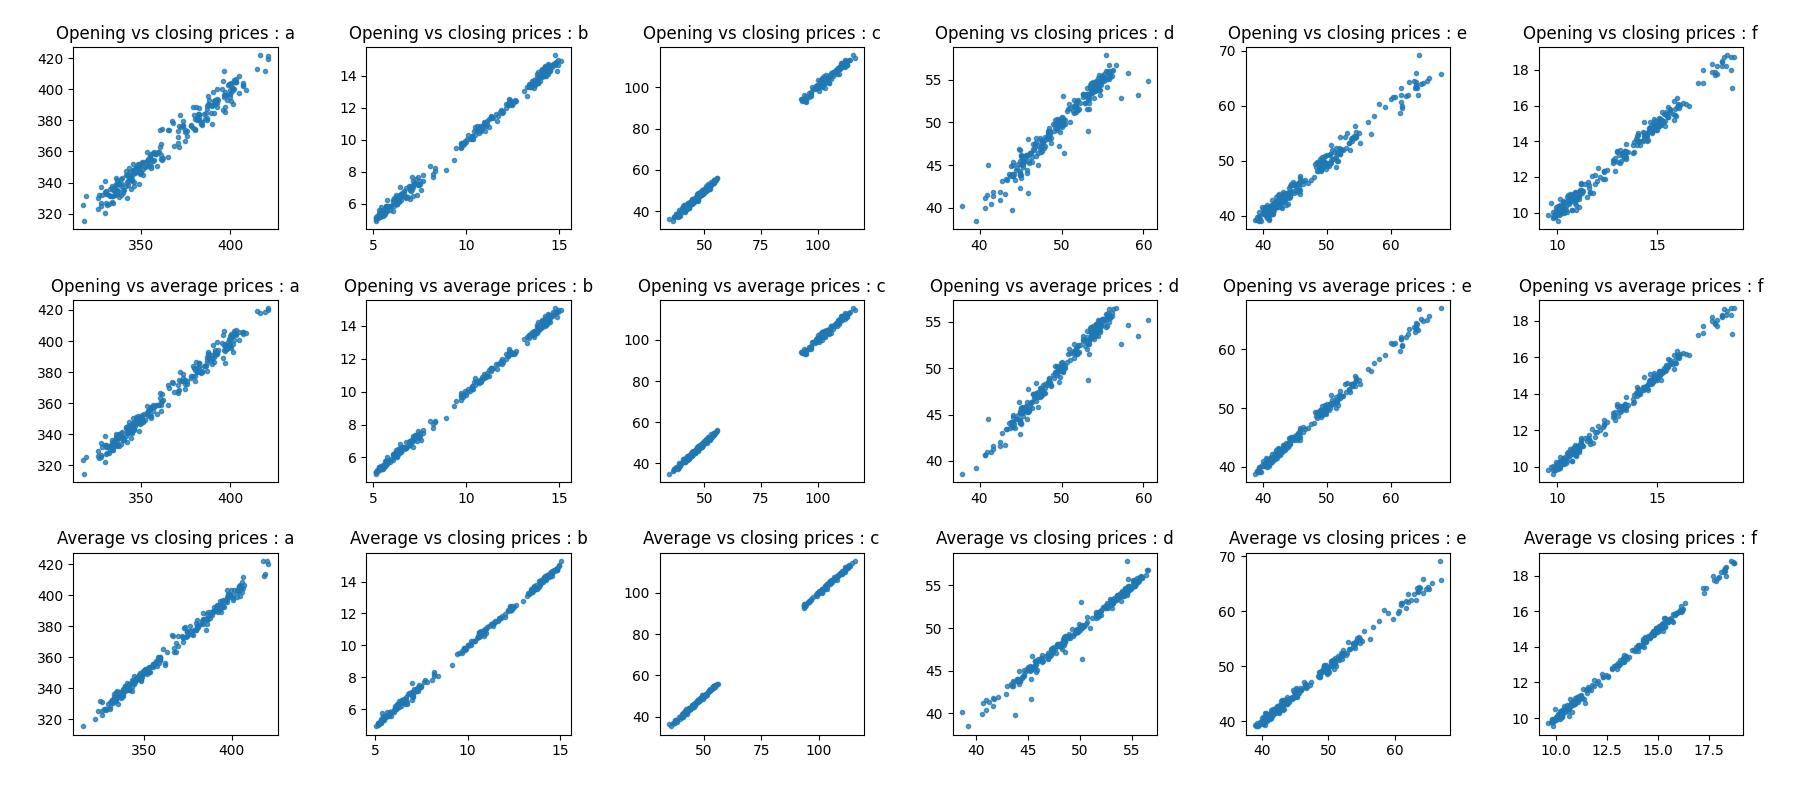
\includegraphics[width=\textwidth, height=0.39\textwidth]{price_choices.jpg}
	\caption{Scatter plots of three natural alternatives for daily price}
	\label{fig5}
\end{figure}

\section{Determining features and target vectors}
We calculate returns for the daily stock prices using two definitions in section 2, the holding period and logarithmic returns. It is interesting to note that when $x$ is small, we have $\log(1+x)\approx x$. This suggests that the two return metrics would be closely related to each other as returns scale over small values. This is confirmed by a plot of the two metrics in aggregated daily data as shown in figure \ref{fig6} where values on the X-axis are trading day counts. 

\begin{figure}[htb]
	\centering
	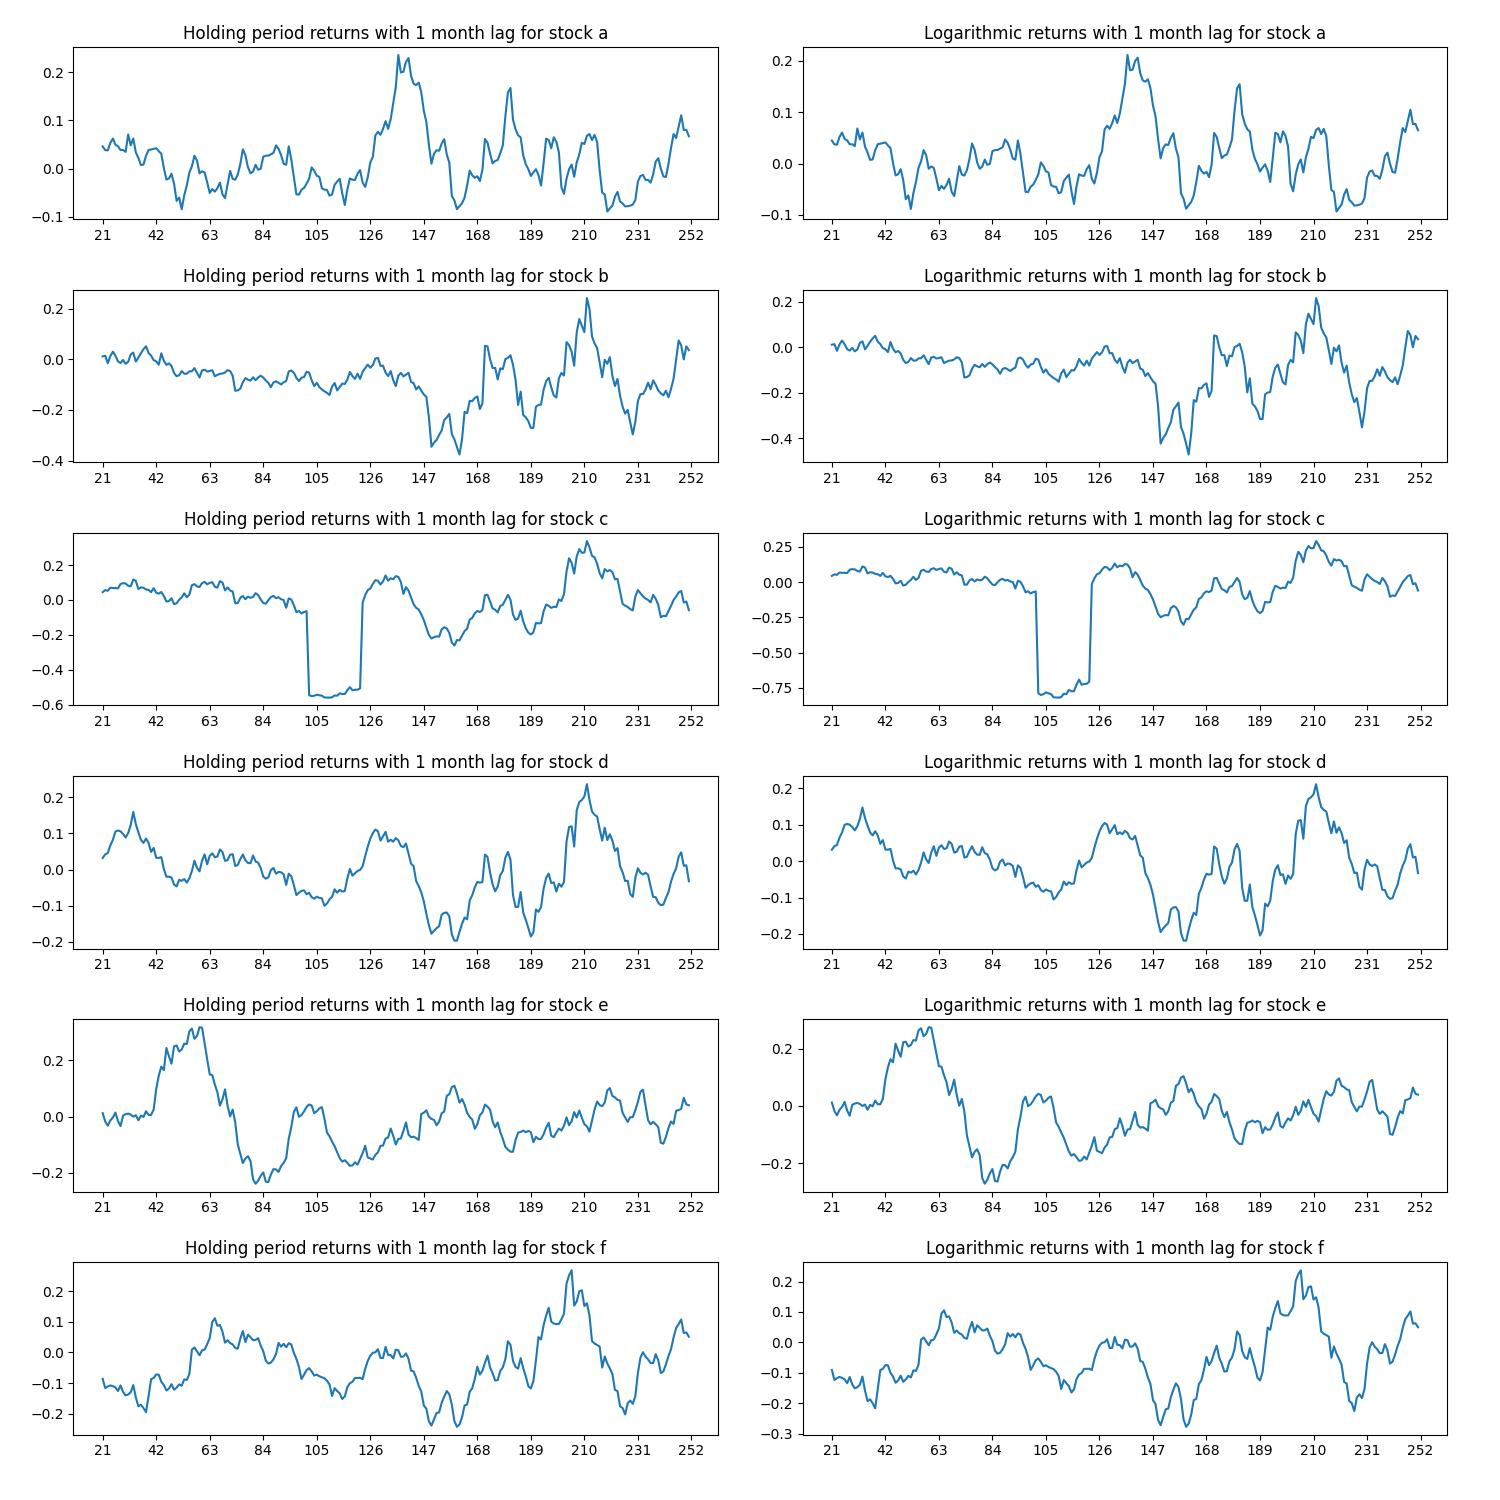
\includegraphics[width=\textwidth]{monthly_returns.jpg}
	\caption{Holding period and logarithmic returns variation over the trading days in a year}
	\label{fig6}
\end{figure}
 
\begin{itemize}
\item Since we could not find obvious time-dependent trends in the data, we will use statistical features which have been historically used for volatility prediction.
\item Our prediction task needs a lead time of 1 month, since we have to predict volatility 1 month into the future. Thus, use of very recent lag features will not be of much help, as we will not have access to those values for the upcoming month. 
\item As suggested in \cite{ghysels2006predicting}, data older than 50 days is not very influential for predicting volatility. That is roughly 2 months. So we build a model that uses a previous month's data as features, leaves a lead time of 1 month and predicts the values for the month after that.
\item Since calculation of returns is done over 1 month, we only have returns data from $2^\text{nd}$ month onward. 
Calculation of volatility from returns is done over 1 month by considering a rolling average, so volatility data is available starting month 3. Thus, the first volatility data that can be in target prediction is from day 1 of month 5.
\end{itemize}
Volatility is calculated as month-long rolling standard deviation in the value of logarithmic returns, and is plotted in figure \ref{fig7} to spot potential trends.

\begin{figure}[htb]
	\centering
	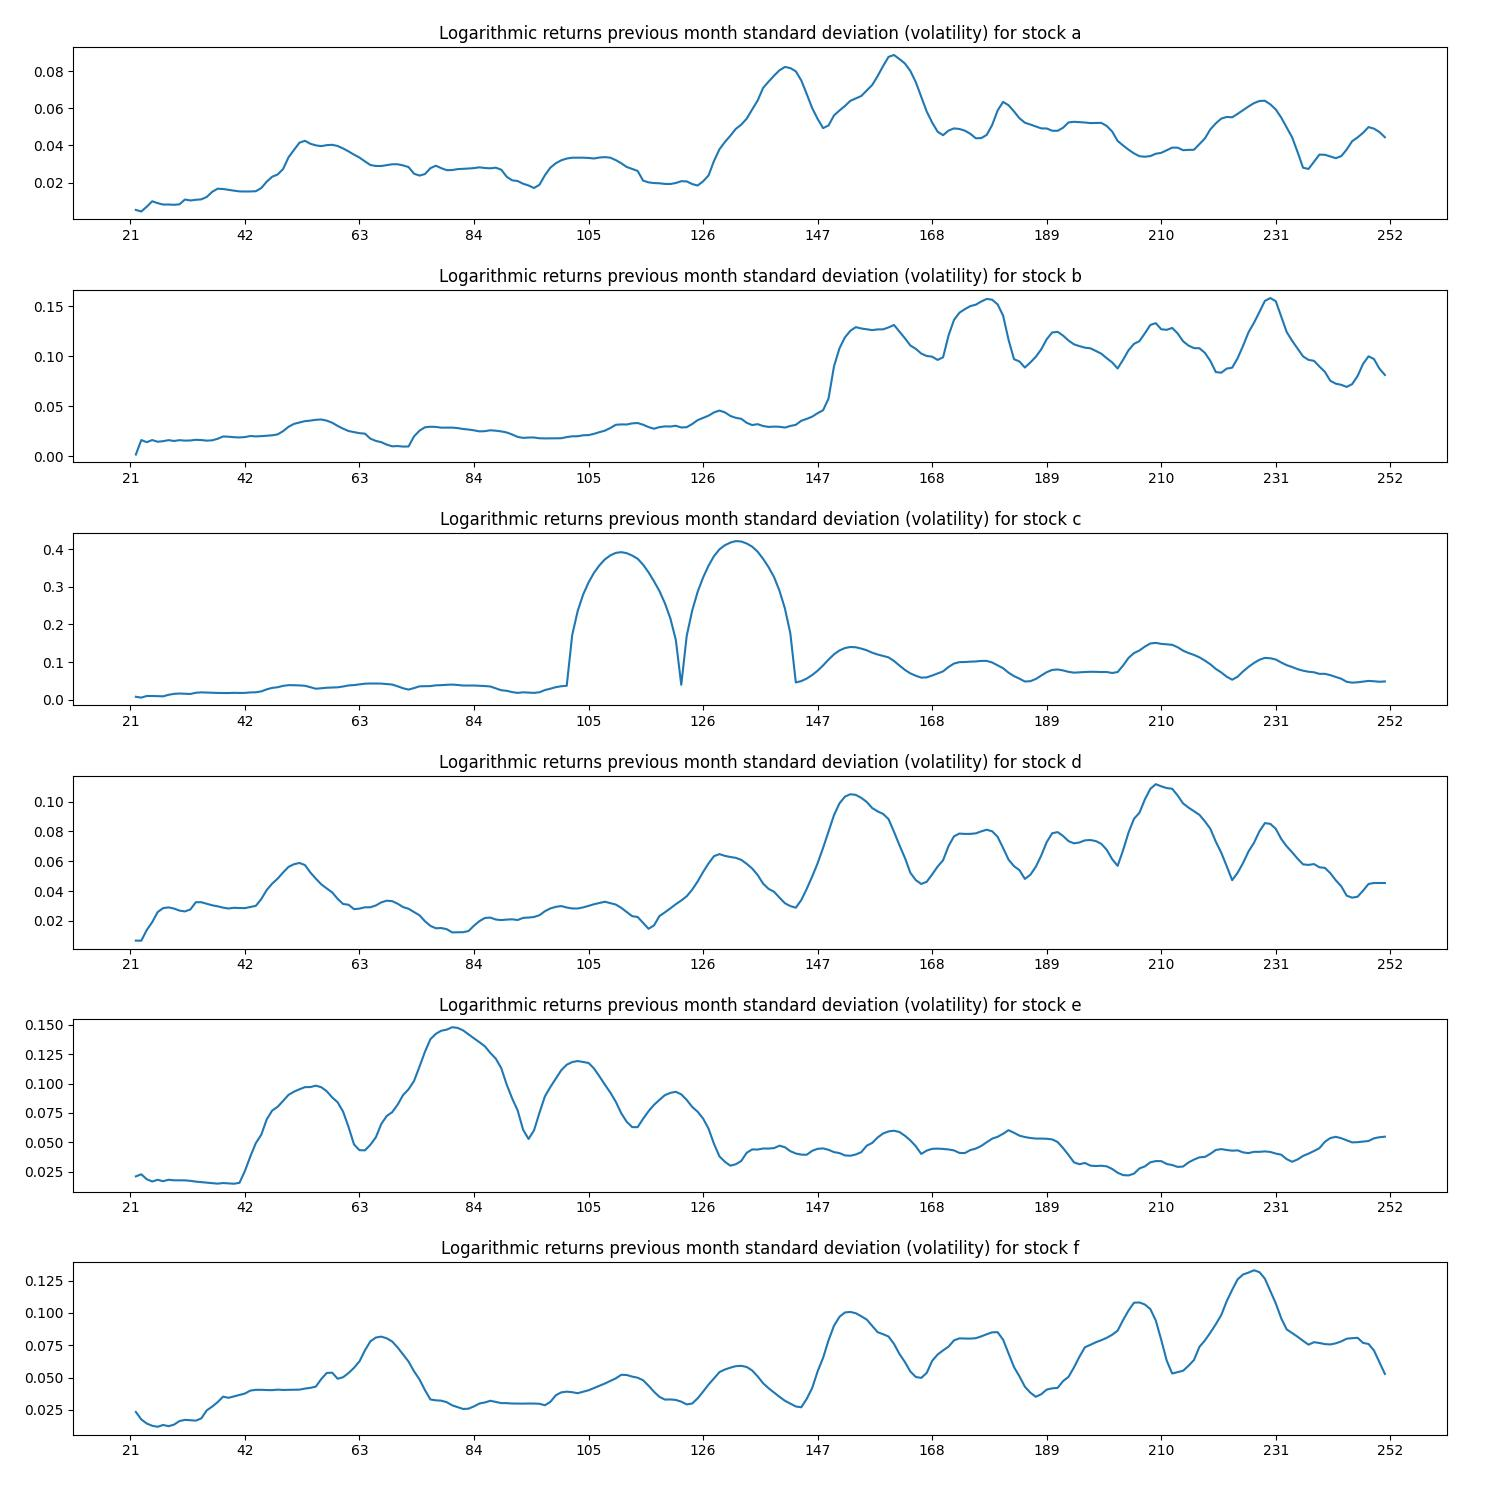
\includegraphics[width=\textwidth, height=0.67\textwidth]{volatility.jpg}
	\caption{Volatility, the monthly rolling standard deviation of $R_\text{log}$}
	\label{fig7}
\end{figure}

\subsection{Feature alternatives}
Referring to multiple highly cited papers on volatility predictions, we obtain ideas to use the following potentially good predictors as features for our data. 
\begin{multicols}{2}
\begin{enumerate}
	\item Square of past returns \cite{bollerslev1987conditionally}
	\item Absolute value of past returns \cite{ding1993long}
	\item Range of past return values (max-min) \cite{alizadeh1999range}
	\item Past values of volatility (lag) \cite{ghysels2006predicting}
	\item Daily range of prices \cite{ghysels2006predicting}
	\item Realized daily power, the sum of intra-daily absolute returns \cite{ghysels2006predicting}
\end{enumerate}
\end{multicols}
Clearly the $5^\text{th}$ and $6^\text{th}$ features require data of higher frequency than daily pricing, so we will only look at the first 4 features as potential predictors moving forward. This is one of the \textbf{trade-offs} for having reduced data frequency to daily. 

\begin{itemize}
	\item It will be interesting to see whether each stock's returns are better determined by considering it as a separate time series, or the data completely flattened into one array for all stocks together in training. To save time in selection of features for specific tasks, we write some handy functions.
\end{itemize}

\section{Models, Training, Validation}
\subsection{Choice of architecture} 
Since financial data typically has trends detectable by simpler models and for the compelling reason of explainability, we use LinearRegression model for all the training. We perform 20-fold cross validation, training a lot of models to fit patterns in the data. The metric chosen for calculating residuals is Mean Squared Error, as recommended in \cite{ghysels2006predicting}. Our goal then is to find the best combination of features to model volatility for the next month.

\subsection{Selecting the best feature combination}
One perk of having easy access to any slices of data with handy functions (mentioned in section 5.1) is that we can train both types of models mentioned earlier (together or separate data for stocks) for a large number of cross validations with mean squared error. Since we have access to 4 features, there are $2^4-1 = 15$ different combinations of them potentially being used as training data. \textbf{We iterate through all these 15 combinations} of features (named $\text{`Data\_presets'}$) during training and save the information for which combination performed the best with a cross entropy validation loss function. 

It is observed that using separate training for each stock results in a smaller mean squared error than the best feature combination for combined data. When using separate data for each stock, the smallest mean square error is obtained for the following combination of features (from section 5.1) -
\begin{multicols}{6}
	\begin{enumerate}[a :]
		\item \{1\}		
		\item \{4\}
		\item \{3,4\}
		\item \{2\}
		\item \{2,4\}
		\item \{3\}
	\end{enumerate}
\end{multicols}

\section{Results}
\begin{itemize}
	\item After finding out the best selection of features for each stock, we train $6$ different linear models that learn volatility information for each stock. 
	\item The relevant feature data for each day of the final month in our data set is then provided as input to the trained model to obtain predictions of volatility for each day of the future month. 
	\item This is different from the exact number "volatility over the next month", which in our definition would simply be the value of volatility value on the last day of the future month. 
	\item We use mean volatility observed over the future month for answering the question of annualized volatility. The answer is obtained by multiplying monthly volatility with $\sqrt{12}$, as discussed in section 2.
	\item The root mean squared error (fluctuation) serves a similar purpose as standard deviation to conclude confidence intervals, so presumably the usual 68-95-99.7 percent confidence rule for 1-2-3 standard deviation applies here as well.
\end{itemize}

\begin{center}
	\def\arraystretch{1.5}
	\begin{tabular}{| c | c | c | c | c | c |}
		\hline
		Stock & Month End Vol. & Month Avg Vol. & M.S. Error & Annualized Vol. & Fluctuation \\ \hline
		a     & 5.04 \%        & 4.62 \%        & 0.000260   & 16.01 \%        & 5.58 \%     \\
		b     & 6.65 \%        & 9.56 \%        & 0.001421   & 33.13 \%        & 13.06 \%    \\
		c     & 17.83 \%       & 10.94 \%       & 0.005972   & 37.91 \%        & 26.77 \%    \\
		d     & 4.16 \%        & 5.93 \%        & 0.000580   & 20.55 \%        & 8.34 \%     \\
		e     & 5.06 \%        & 4.39 \%        & 0.000256   & 15.21 \%        & 5.54 \%     \\
		f     & 6.98 \%        & 7.72  \%       & 0.000684   & 26.74 \%        & 9.06 \%     \\ \hline
	\end{tabular}
\end{center}	

\section{Limitations, future improvements}
 The fluctuations in result coming from root mean squared error seem to be high, which means the confidence intervals are really wide in this current result. I believe the use of a smarter error metric or better calculation of the error than 95\% of training data (coming from 20-fold cross validation) can improve these results and provide a more confident estimation of volatility.

\bibliographystyle{abbrv}
\bibliography{sources}
\pagebreak

\section{Appendix : Explainability of the linear model}

As mentioned in section 6.1, the linear model is simple to explain. As observed commonly from the plots here for regression coefficients, more recent data plays a more crucial role in predicting volatility. There also seem to be some periodicity in coefficients along training time horizon.

\begin{figure}[htb]
	\centering
	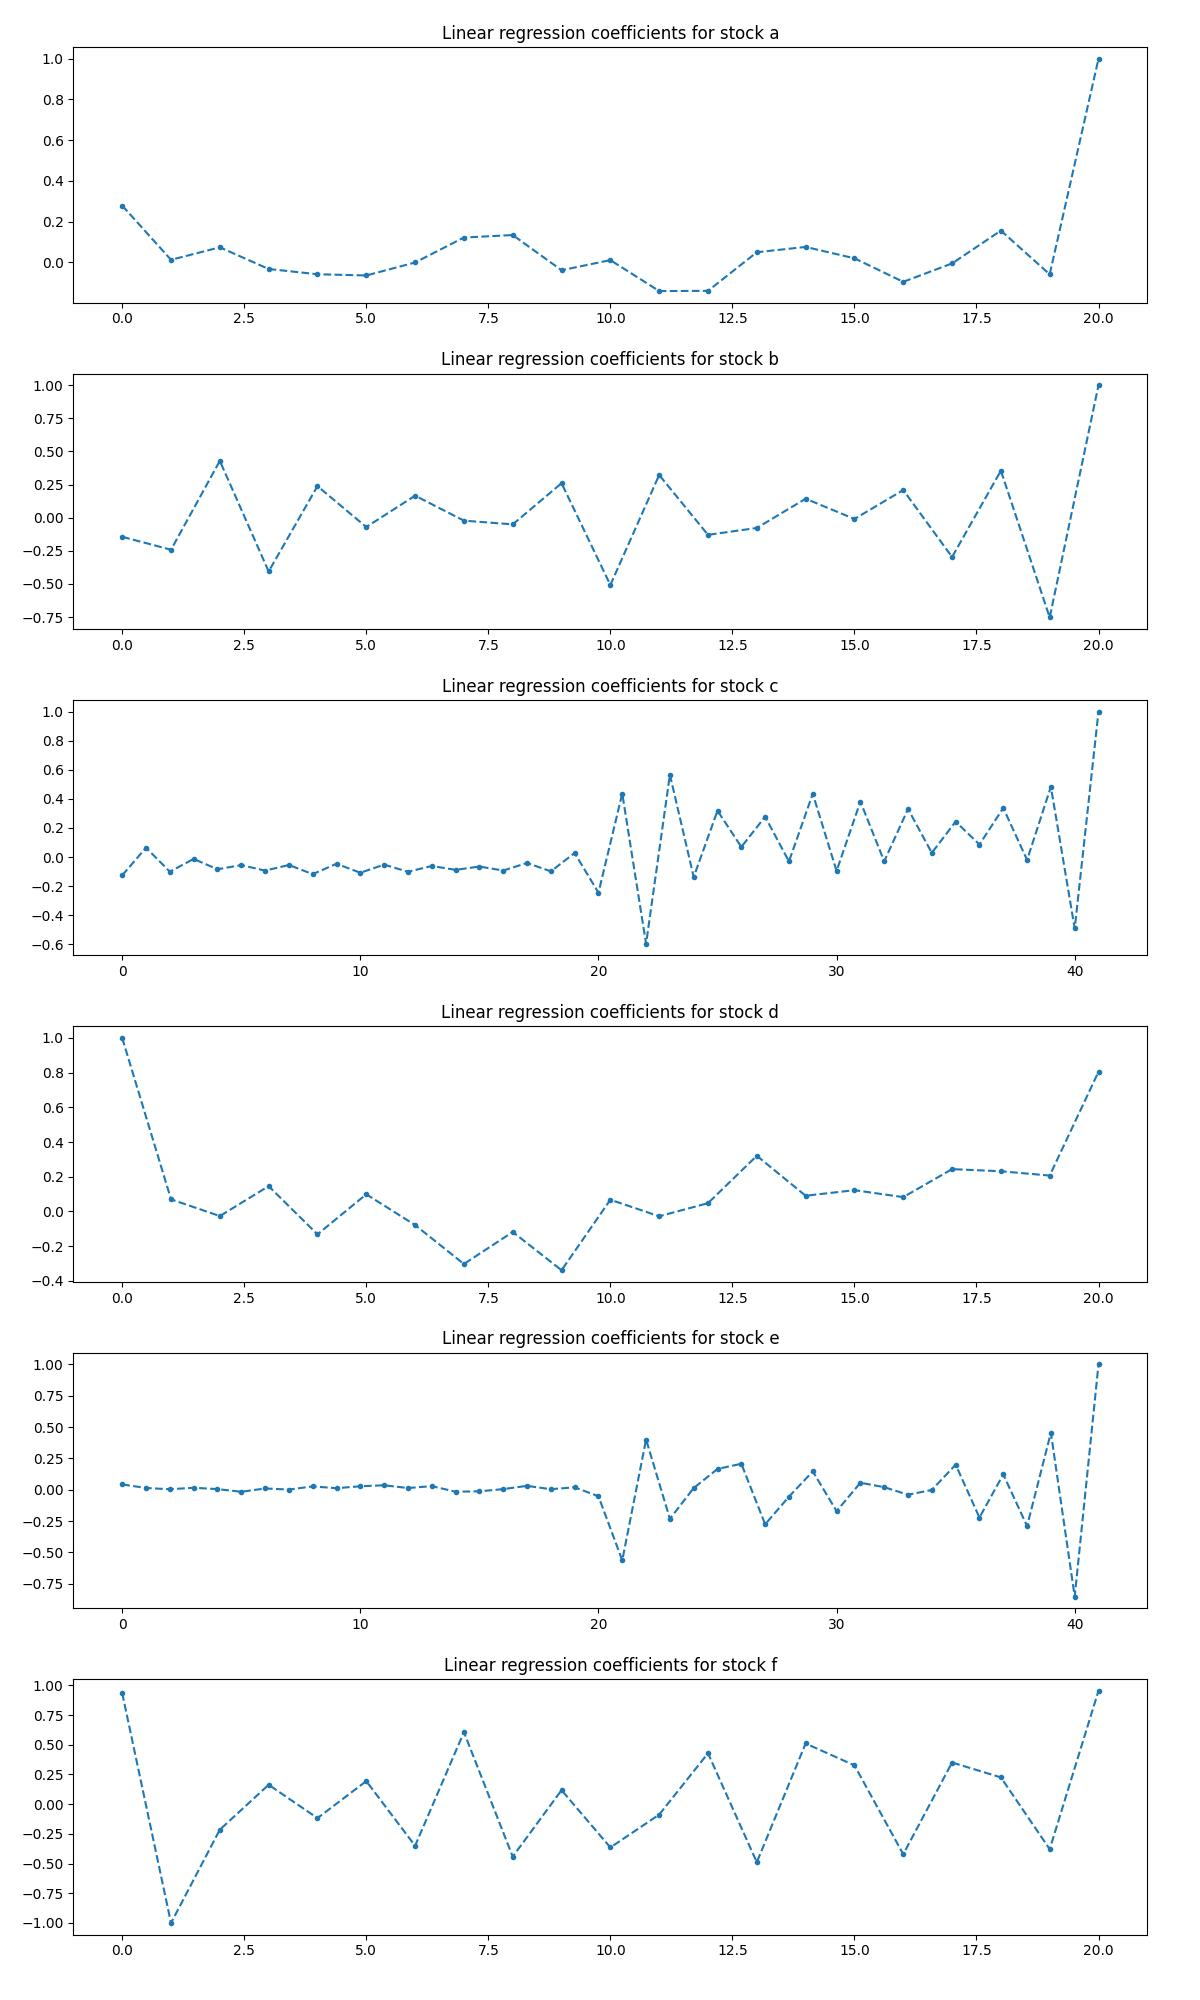
\includegraphics[width=0.6\textwidth, ]{model_coeffs.jpg}
	\caption{Regression coefficients normalized in $(-1,1)$ range}
	\label{fig8}
\end{figure}	

\end{document}